% =====================================================================
%  Portafolio de proyectos — Rodrigo Yupanqui Rubio
%  Compilar con:  pdflatex portafolio.tex  (dos pasadas)
% =====================================================================
\documentclass[10pt,a4paper]{article}

\usepackage[utf8]{inputenc}
\usepackage[T1]{fontenc}
\usepackage[spanish,es-noshorthands]{babel}
\usepackage{lmodern}
\usepackage[a4paper,margin=1.35cm,top=1.2cm,bottom=1.1cm]{geometry}
\usepackage{amsmath,amssymb}
\usepackage{graphicx}
\usepackage{booktabs,array,tabularx}
\usepackage[table]{xcolor}
\usepackage{tikz}
\usetikzlibrary{arrows.meta,positioning,shapes.misc,fit,backgrounds}
\usepackage[most]{tcolorbox}
\usepackage{enumitem}
\usepackage{microtype}
\usepackage{caption}
\usepackage{fontawesome5}
\usepackage[colorlinks=true,urlcolor=accent,linkcolor=accent]{hyperref}

\renewcommand{\familydefault}{\sfdefault}
\pagestyle{empty}
\setlength{\parindent}{0pt}
\setlength{\parskip}{4pt}
\captionsetup{font={footnotesize,it},labelformat=empty,skip=2pt,justification=centering}
\setlist{nosep,leftmargin=1.1em,itemsep=1.5pt}

% ---------- Paleta ----------
\definecolor{ink}{RGB}{16,24,40}
\definecolor{accent}{RGB}{0,98,163}
\definecolor{accent2}{RGB}{232,119,34}
\definecolor{soft}{RGB}{238,243,249}
\definecolor{rule}{RGB}{200,210,222}
\color{ink}

% ---------- Macros ----------
\newcommand{\sect}[1]{\par\vspace{5pt}{\color{accent}\bfseries\large #1}\par\vspace{1pt}{\color{rule}\hrule height 0.6pt}\vspace{4pt}}

% Cabecera de proyecto: numero, titulo, subtitulo
\newcommand{\projecthead}[3]{%
  \begin{tcolorbox}[enhanced,colback=accent,colframe=accent,arc=3pt,boxrule=0pt,
      left=8pt,right=8pt,top=5pt,bottom=5pt,
      overlay={\node[anchor=east,text=white,opacity=0.18,font=\fontsize{46}{46}\selectfont\bfseries] at ([xshift=-8pt]frame.east) {#1};}]
    {\color{white}\Large\bfseries #2}\\[-1pt]
    {\color{white}\small #3}
  \end{tcolorbox}\vspace{-4pt}}

% Franja de metricas: cuatro cajas  {valor}{etiqueta}
\newcommand{\metric}[2]{%
  \begin{tcolorbox}[colback=soft,colframe=soft,boxrule=0pt,arc=2pt,left=2pt,right=2pt,top=2pt,bottom=2pt,
      width=\linewidth,halign=center,nobeforeafter]
    {\color{accent}\large\bfseries #1}\\[-2pt]{\scriptsize #2}
  \end{tcolorbox}}
\newcommand{\metricstrip}[8]{%
  \begin{tabularx}{\linewidth}{@{}X@{\hspace{4pt}}X@{\hspace{4pt}}X@{\hspace{4pt}}X@{}}
    \metric{#1}{#2} & \metric{#3}{#4} & \metric{#5}{#6} & \metric{#7}{#8}
  \end{tabularx}\par\vspace{1pt}}

\newcommand{\rolebox}[1]{%
  \begin{tcolorbox}[colback=white,colframe=accent2,boxrule=0.8pt,leftrule=3pt,arc=2pt,
      left=5pt,right=5pt,top=3pt,bottom=3pt,title={\small\bfseries Mi aporte},
      coltitle=white,colbacktitle=accent2,fonttitle=\bfseries\small,attach boxed title to top left={xshift=6pt,yshift=-2mm},boxed title style={arc=2pt,boxrule=0pt,top=0.5pt,bottom=0.5pt}]
    \small #1
  \end{tcolorbox}}

\begin{document}

% =====================================================================
%  PORTADA
% =====================================================================
\begin{tcolorbox}[enhanced,colback=ink,colframe=ink,arc=4pt,boxrule=0pt,left=14pt,right=14pt,top=12pt,bottom=12pt]
  {\color{white}\fontsize{27}{30}\selectfont\bfseries Rodrigo Yupanqui Rubio}\\[3pt]
  {\color{accent2}\large\bfseries Ingeniería Electrónica \;$\cdot$\; Sistemas embebidos, IoT e instrumentación}\\[6pt]
  {\color{white}\small
    \faEnvelope\;\href{mailto:rodrigo.yupanqui@pucp.edu.pe}{\textcolor{white}{rodrigo.yupanqui@pucp.edu.pe}}\quad
    \faLinkedin\;\href{https://www.linkedin.com/in/rodrigo-yupanqui/}{\textcolor{white}{linkedin.com/in/rodrigo-yupanqui}}\quad
    \faGithub\;\href{https://github.com/RodrigoYupanqui}{\textcolor{white}{github.com/RodrigoYupanqui}}\quad
    \faMapMarker*\; Lima, Perú}
\end{tcolorbox}

\vspace{-2pt}
\sect{Perfil}
Estudiante de Ingeniería Electrónica en la \textbf{Pontificia Universidad Católica del Perú (PUCP)}, ubicado en el
\textbf{5\,\% superior de Ingeniería Electrónica} y en el \textbf{10\,\% superior de la Facultad de Ciencias e Ingeniería}.
Practicante de Ingeniería Electrónica en \textbf{DIACSA} (sensores, firmware, instrumentación, adquisición de datos e integración de hardware).
Transformo requisitos de ingeniería en prototipos funcionales combinando electrónica, firmware, integración mecánica y procesamiento de datos.

\vspace{2pt}
\begin{minipage}[t]{0.485\linewidth}
\sect{Capacidades técnicas}
\renewcommand{\arraystretch}{1.25}
\footnotesize
\begin{tabularx}{\linewidth}{@{}>{\bfseries\color{accent}}p{2.3cm}X@{}}
Firmware       & C/C++, Arduino-ESP32 (FreeRTOS, ISR, temporizadores), Python\\
Plataformas    & ESP32, ESP32-S3, STM32, Arduino, Raspberry Pi 4B/5\\
Conectividad   & LoRa (SX1278), Wi-Fi, WebSocket seguro (WSS), UART, I\textsuperscript{2}C, SPI, I\textsuperscript{2}S\\
Sensórica      & IMU, magnetómetro, GPS, BME280, INA219, LiDAR, cámaras, encoders\\
Control        & Regulación PI con \emph{anti-windup}, filtrado EMA, PWM, servos\\
Visión / IA    & OpenCV, YOLOv11n en el borde, segmentación HSV, nubes de puntos\\
Diseño HW      & EasyEDA, LTspice, Proteus, Inventor, AutoCAD, PCB a medida\\
Software       & FastAPI, Next.js, Git/GitHub, Linux, MATLAB, NumPy/Pandas\\
\end{tabularx}
\end{minipage}\hfill
\begin{minipage}[t]{0.485\linewidth}
\sect{Experiencia y liderazgo}
\small
\begin{itemize}
  \item \textbf{DIACSA} — Practicante de Ingeniería Electrónica.
  \item \textbf{IEEE Computer Society PUCP} — Director de Proyectos; liderazgo de equipos multidisciplinarios.
  \item \textbf{Huawei Seeds for the Future} — participante seleccionado.
  \item \textbf{Siemens, Programa Regional de Eficiencia Energética} — análisis de optimización energética.
  \item Instructor voluntario en talleres de electrónica.
  \item \textbf{Co-autor} del manuscrito sobre CrackScan (PUCP, Laboratorio de Procesamiento Digital de Señales).
  \item Finalista (17 equipos) en la \textbf{Primera Competencia Nacional de Pequeños Satélites 2024}.
\end{itemize}
\end{minipage}

\sect{Mapa de capacidades IoT demostradas en los proyectos}
\renewcommand{\arraystretch}{1.22}
\footnotesize
\rowcolors{2}{soft}{white}
\begin{tabularx}{\linewidth}{@{}>{\bfseries}p{3.45cm}XXX@{}}
\rowcolor{accent}\color{white}Capacidad & \color{white}\bfseries 1 \; CrackScan & \color{white}\bfseries 2 \; CubeSat & \color{white}\bfseries 3 \; Arpeggiator\\
Adquisición multisensor        & Encoders, LiDAR, cámaras, GPS         & 6 sensores en bus I\textsuperscript{2}C + UART & 13 entradas, 2 ADC\\
Comunicación inalámbrica       & WSS/JSON, telemetría a 1~Hz          & LoRa 433~MHz, paquetes de 50 car.              & --- \\
Comunicación entre nodos       & UART 115\,200~baud con \emph{timeout} & Enlace TX/RX ESP32--ESP32                       & I\textsuperscript{2}S a DAC\\
Control en lazo cerrado        & PI de velocidad, lazo de 100~ms        & Despliegue por altitud con histéresis           & Filtro IIR 1.er orden\\
Edge AI / procesamiento        & YOLOv11n en RPi\,5, RANSAC            & Altitud barométrica                             & Síntesis por LUT\\
Diseño de PCB y mecánica       & PCB propia, chasis 4 ruedas            & 2 PCB (EasyEDA) en estructura 1U                & PCB doble capa, MDF\\
Interfaz de monitoreo          & Dashboard web (PWA)                   & GUI de estación terrena                         & LEDs WS2812B\\
\end{tabularx}
\rowcolors{1}{white}{white}

\sect{Proyectos destacados}
\begin{tabularx}{\linewidth}{@{}XXX@{}}
\begin{minipage}[t]{0.97\linewidth}\centering
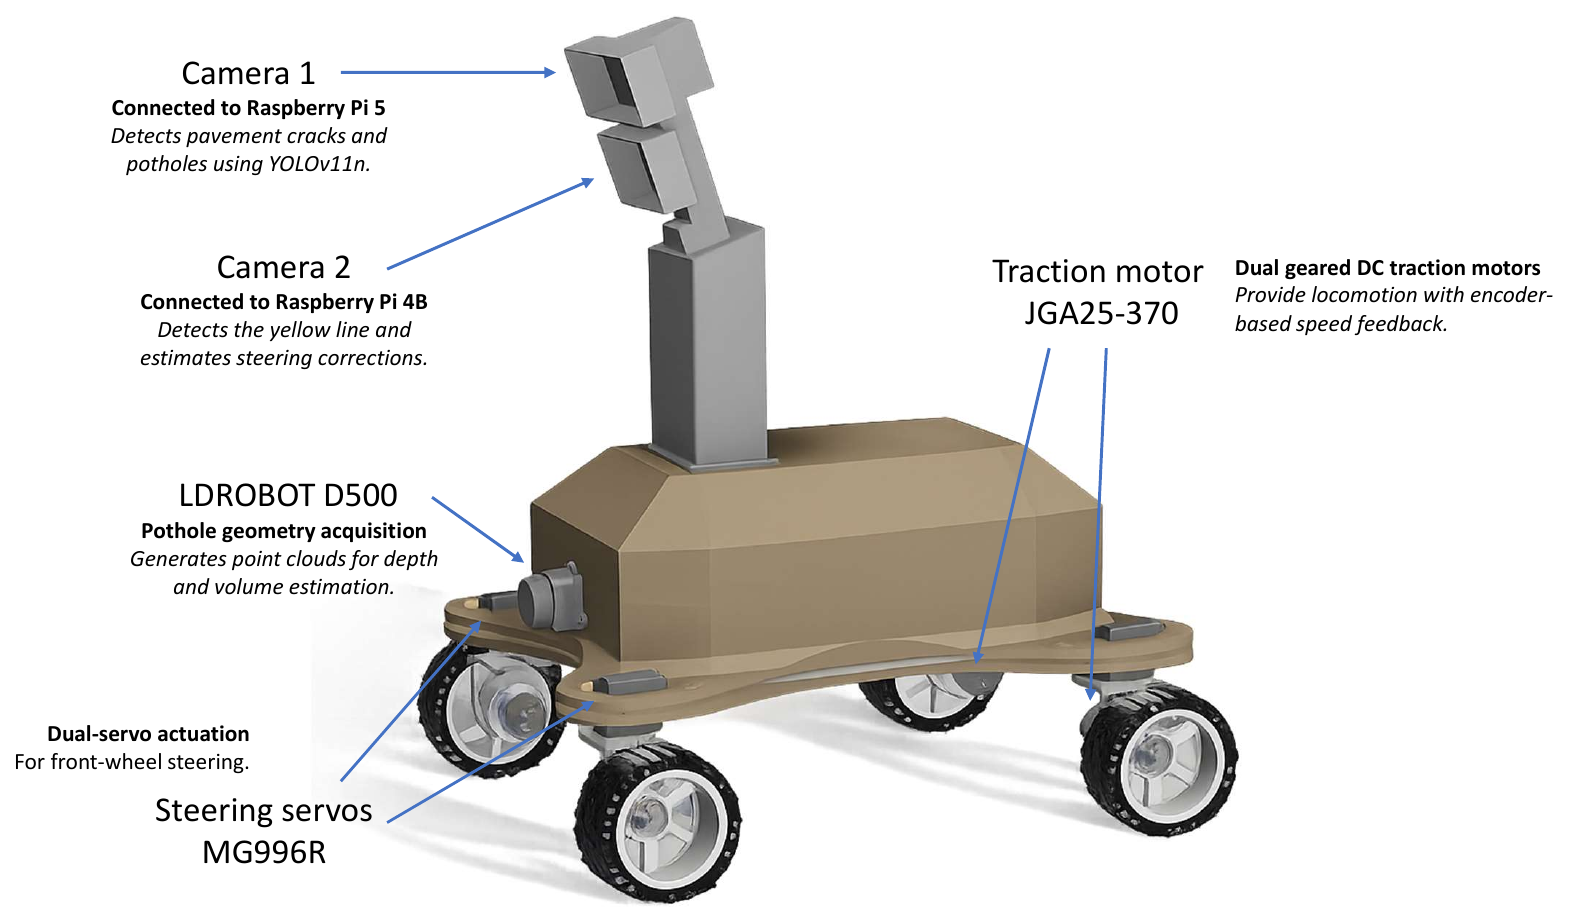
\includegraphics[width=\linewidth,height=3.1cm,keepaspectratio]{img/rover-render.png}\\[2pt]
{\bfseries\color{accent}01 \; \href{https://github.com/RodrigoYupanqui/CrackScan}{CrackScan}}\\[1pt]
{\footnotesize Rover autónomo con YOLOv11n, LiDAR y navegación visual; control distribuido en 3 nodos. \emph{Co-autor de manuscrito.}}
\end{minipage} &
\begin{minipage}[t]{0.97\linewidth}\centering
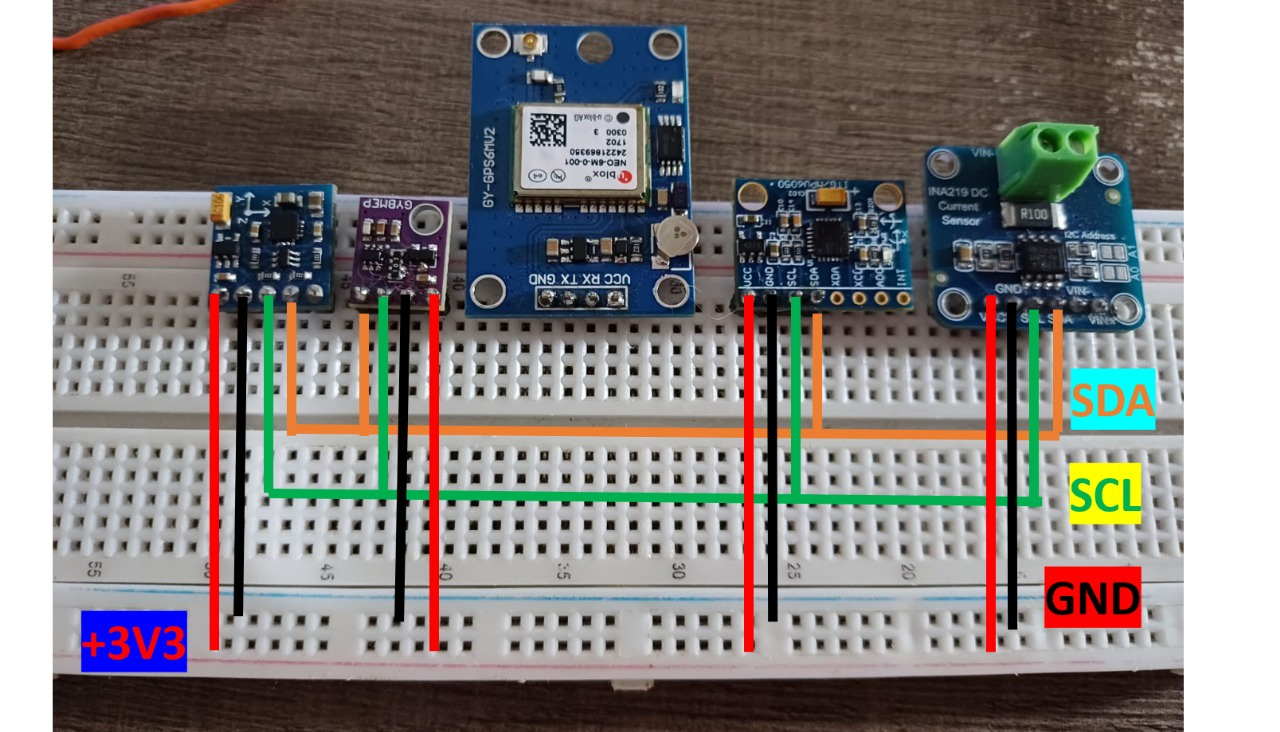
\includegraphics[width=\linewidth,height=3.1cm,keepaspectratio]{img/cs_Cmlhuhz.jpeg}\\[2pt]
{\bfseries\color{accent}02 \; \href{https://github.com/RodrigoYupanqui/CubeSat}{CubeSat 1U}}\\[1pt]
{\footnotesize Telemetría LoRa de 21 variables, 6 sensores y despliegue de paracaídas por altitud. \emph{Finalista nacional (17 equipos).}}
\end{minipage} &
\begin{minipage}[t]{0.97\linewidth}\centering
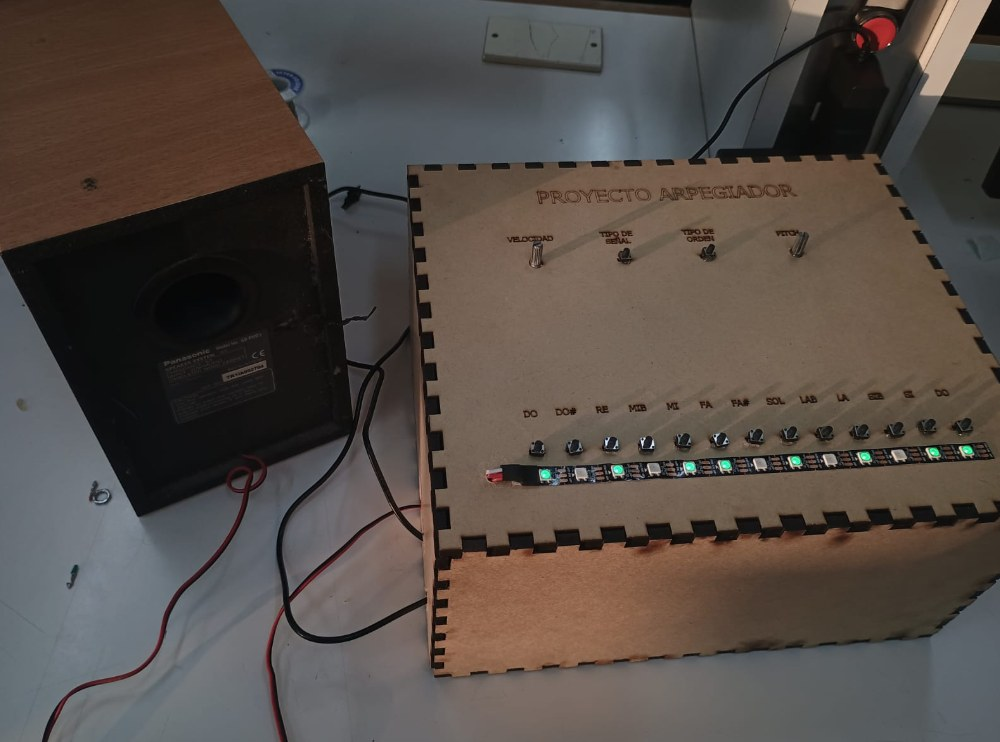
\includegraphics[width=\linewidth,height=3.1cm,keepaspectratio]{img/arp_final-prototype.jpg}\\[2pt]
{\bfseries\color{accent}03 \; \href{https://github.com/RodrigoYupanqui/Arpeggiator}{Arpeggiator}}\\[1pt]
{\footnotesize Instrumento musical ESP32-S3 con audio I\textsuperscript{2}S, PCB propia y gabinete en MDF. \emph{De la idea al producto.}}
\end{minipage}
\end{tabularx}

\sect{Qué aporto a un proyecto IoT}
\small
\begin{tabularx}{\linewidth}{@{}XX@{}}
\begin{minipage}[t]{0.97\linewidth}
\begin{itemize}
  \item \textbf{Capa de dispositivo:} selección de componentes, esquemáticos, PCB y firmware robusto (ISR, temporizadores, \emph{timeouts} de seguridad).
  \item \textbf{Capa de conectividad:} LoRa, Wi-Fi, WSS, UART, I\textsuperscript{2}C/SPI/I\textsuperscript{2}S; protocolos propios documentados.
\end{itemize}
\end{minipage} &
\begin{minipage}[t]{0.97\linewidth}
\begin{itemize}
  \item \textbf{Capa de datos y nube:} telemetría JSON, servidor FastAPI, dashboard web y estaciones de monitoreo.
  \item \textbf{Edge AI y validación:} inferencia en el borde, métricas reportadas (mAP, F1, FPS) y documentación técnica rigurosa.
\end{itemize}
\end{minipage}
\end{tabularx}


\newpage

% =====================================================================
%  PROYECTO 1 — CRACKSCAN
% =====================================================================
\projecthead{01}{CrackScan — Rover autónomo de inspección de pavimentos}
  {Visión por computador $\cdot$ LiDAR $\cdot$ control embebido distribuido \;|\; Proyecto Electrónico 1 (2025-1), PUCP \;|\; Asesor: S.\,E.~Romero}

\metricstrip{0.78}{mAP@0.5 (YOLOv11n)}{6.10 FPS}{inferencia en RPi\,5 (163.8 ms)}{7123 pts}{nube LiDAR en 0.40 s}{0\,\%}{intervención manual (pista evaluada)}

\begin{minipage}[t]{0.545\linewidth}
\vspace{0pt}
\sect{Descripción}
Rover de bajo costo (componentes COTS) que \textbf{detecta grietas y baches, reconstruye en 3D los baches detectados y navega
siguiendo una línea amarilla}. Arquitectura distribuida de tres nodos:
\begin{itemize}
  \item \textbf{Raspberry Pi 5}: YOLOv11n (grietas/baches), activación \emph{selectiva} del LiDAR LDROBOT D500, volumen del bache, servidor FastAPI.
  \item \textbf{Raspberry Pi 4B}: segmentación HSV de la línea, ROI trapezoidal, centroide ponderado y ángulo de corrección a $\approx$20~Hz.
  \item \textbf{ESP32-WROOM-32U}: PI de velocidad de 2 motores, 2 servos de dirección sincronizados, WSS y telemetría.
\end{itemize}

\sect{Detalles técnicos}
\textbf{Control de motores} (cada 100~ms, $T_s=0.1$~s, 1050 pulsos/vuelta):
\begin{align}
  \omega[k] &= \frac{600\,n_\mathrm{enc}[k]}{1050}\;\mathrm{RPM},\qquad e[k]=\omega^{*}-\omega[k]\\
  I[k] &= \operatorname{sat}_{[0,255]}\!\big(I[k-1]+K_i\,e[k]\,T_s\big)\\
  u[k] &= \operatorname{sat}_{[0,255]}\!\big(K_p\,e[k]+I[k]\big)
\end{align}
con $K_p=1.8$, $K_i=3.2$ y \emph{anti-windup} por saturación del integrador.

\textbf{Dirección autónoma}: ángulo recibido por UART (\texttt{A:<ang>,V:<ok>}), recortado a $\pm45^\circ$ y suavizado con EMA:
\begin{equation}
  \theta_f[k]=(1-\alpha)\,\theta_f[k-1]+\alpha\,\theta[k],\qquad \alpha=0.25
\end{equation}
con banda muerta de $1^\circ$, servos limitados a $60^\circ$--$120^\circ$ y \textbf{parada de seguridad} si el enlace UART calla $>200$~ms.

\textbf{Volumen del bache}: plano de referencia por RANSAC y mapa de profundidad $d_{ij}$ en rejilla regular:
$\;V=\sum_{i,j} d_{ij}\,\Delta A_{ij}$.

\renewcommand{\arraystretch}{1.12}\footnotesize
\begin{tabularx}{\linewidth}{@{}>{\bfseries}lXr@{}}
\toprule
Clase & Precisión / Recall / F1 & FN\\\midrule
Grietas & 0.84 / 0.87 / 0.85 & 83\\
Baches  & 0.71 / 0.76 / 0.74 & 186\\\bottomrule
\end{tabularx}
\captionsetup{font=scriptsize}\vspace{-1pt}
{\scriptsize Entrenado con 7244 imágenes; prueba con 265 imágenes (640$\times$480).}

\sect{Interfaces y protocolos}
\footnotesize\renewcommand{\arraystretch}{1.12}
\begin{tabularx}{\linewidth}{@{}>{\bfseries\raggedright\arraybackslash}p{2.35cm}>{\raggedright\arraybackslash}X@{}}
\toprule
RPi\,4B$\to$ESP32 & UART 115\,200~baud, 8N1: \texttt{A:-21.20,V:1}; \texttt{START\_AUTO}/\texttt{STOP\_AUTO} en sentido inverso.\\
Backend$\leftrightarrow$ESP32 & WSS (443, \texttt{/ws}) con JSON: \texttt{control}, \texttt{navigation}, \texttt{navigation\_target}; telemetría \texttt{sensor} a $\approx$1~Hz.\\
Seguridad & Credenciales fuera del repositorio (\texttt{secrets.h}); parada a velocidad cero ante pérdida de enlace.\\\bottomrule
\end{tabularx}

\sect{Resultados y análisis crítico}
\small
\begin{itemize}
  \item Navegación continua con detección válida de la línea en la pista evaluada, \textbf{sin intervención manual}.
  \item Los \textbf{falsos negativos de baches (186)} son el modo de fallo crítico: inhiben el LiDAR selectivo. La validación del volumen contra una medición física queda como trabajo siguiente.
\end{itemize}
\end{minipage}\hfill
\begin{minipage}[t]{0.435\linewidth}
\vspace{0pt}
\centering
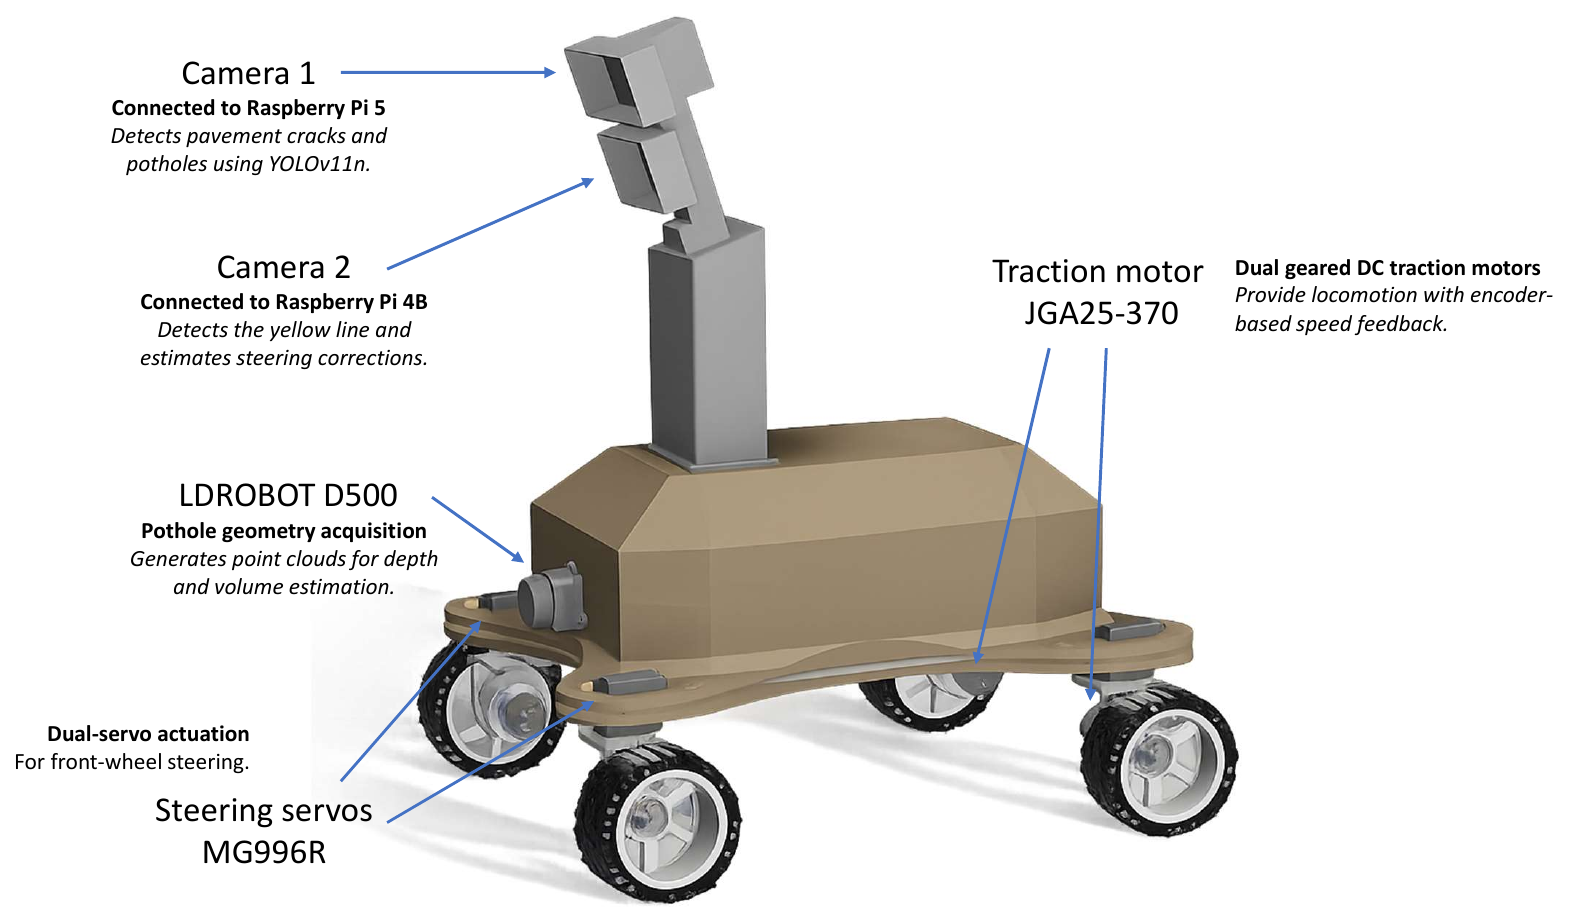
\includegraphics[width=\linewidth]{img/rover-render.png}
\captionof{figure}{Plataforma: cámaras, LiDAR D500, tracción JGA25-370 y dirección con 2 servos MG996R.}
\vspace{3pt}
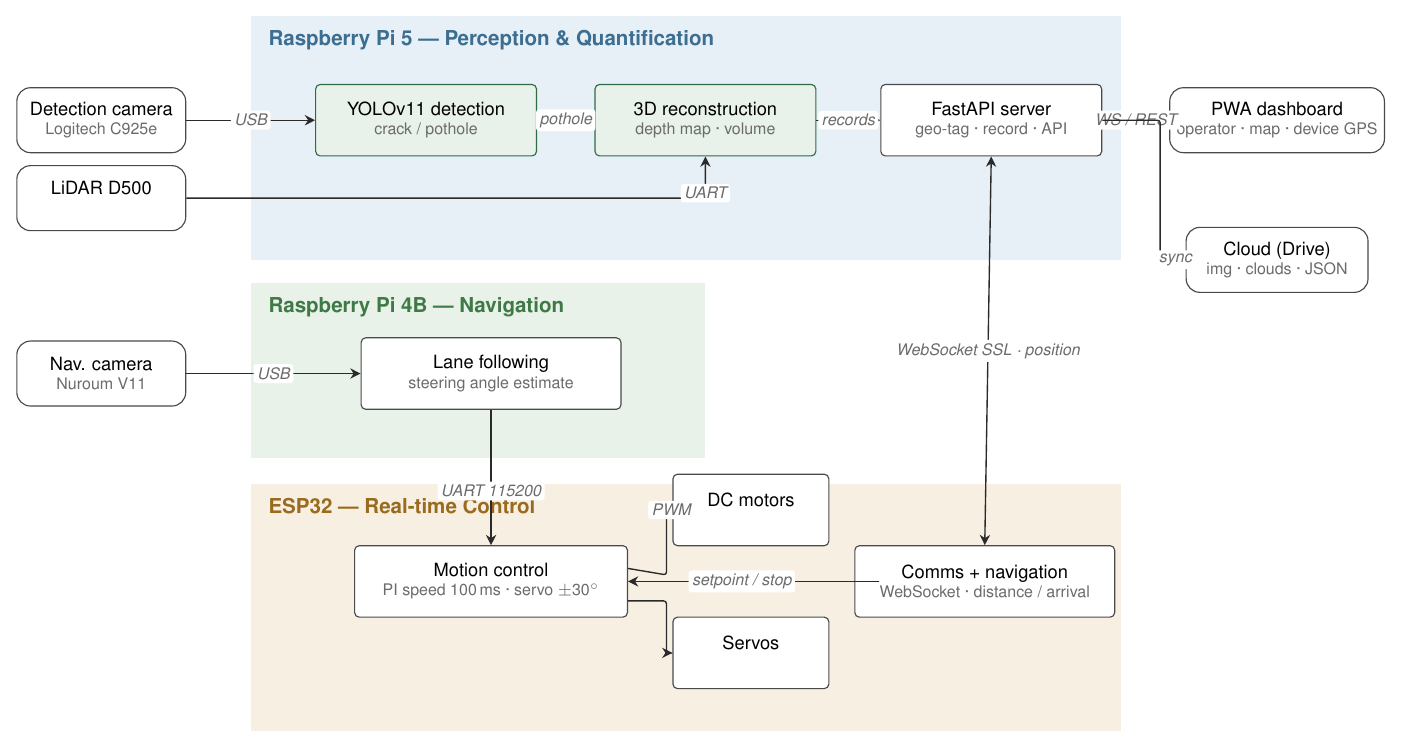
\includegraphics[width=\linewidth]{img/software-architecture.png}
\captionof{figure}{Arquitectura de software distribuida (RPi\,5, RPi\,4B, ESP32).}
\vspace{3pt}
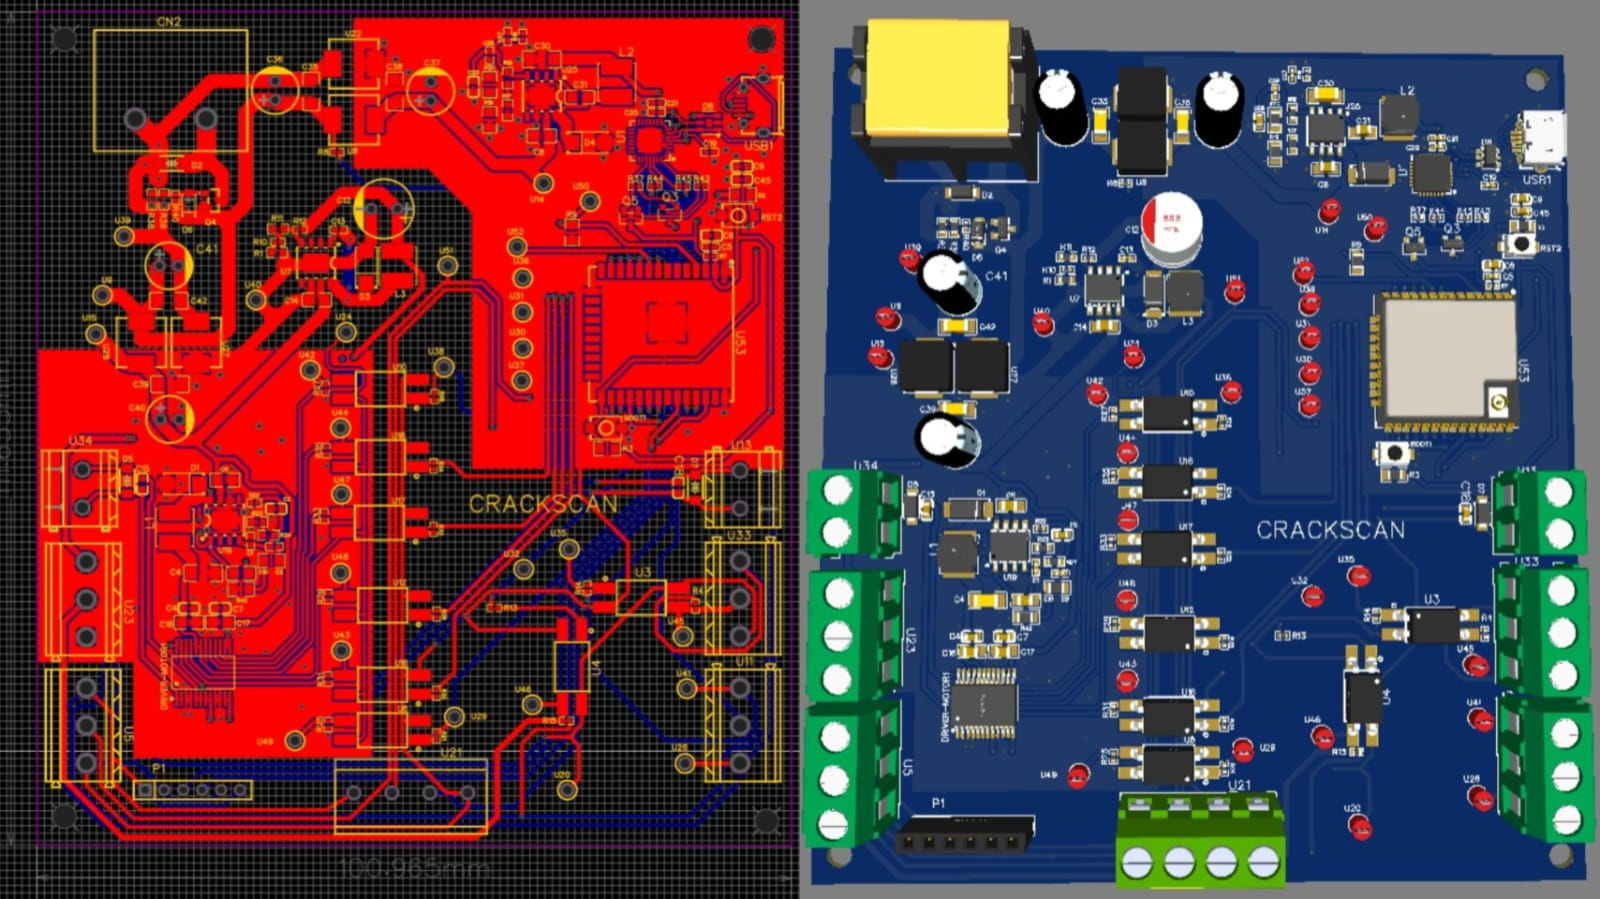
\includegraphics[width=\linewidth]{img/pcb-design.png}
\captionof{figure}{PCB propia de integración electrónica.}
\vspace{3pt}
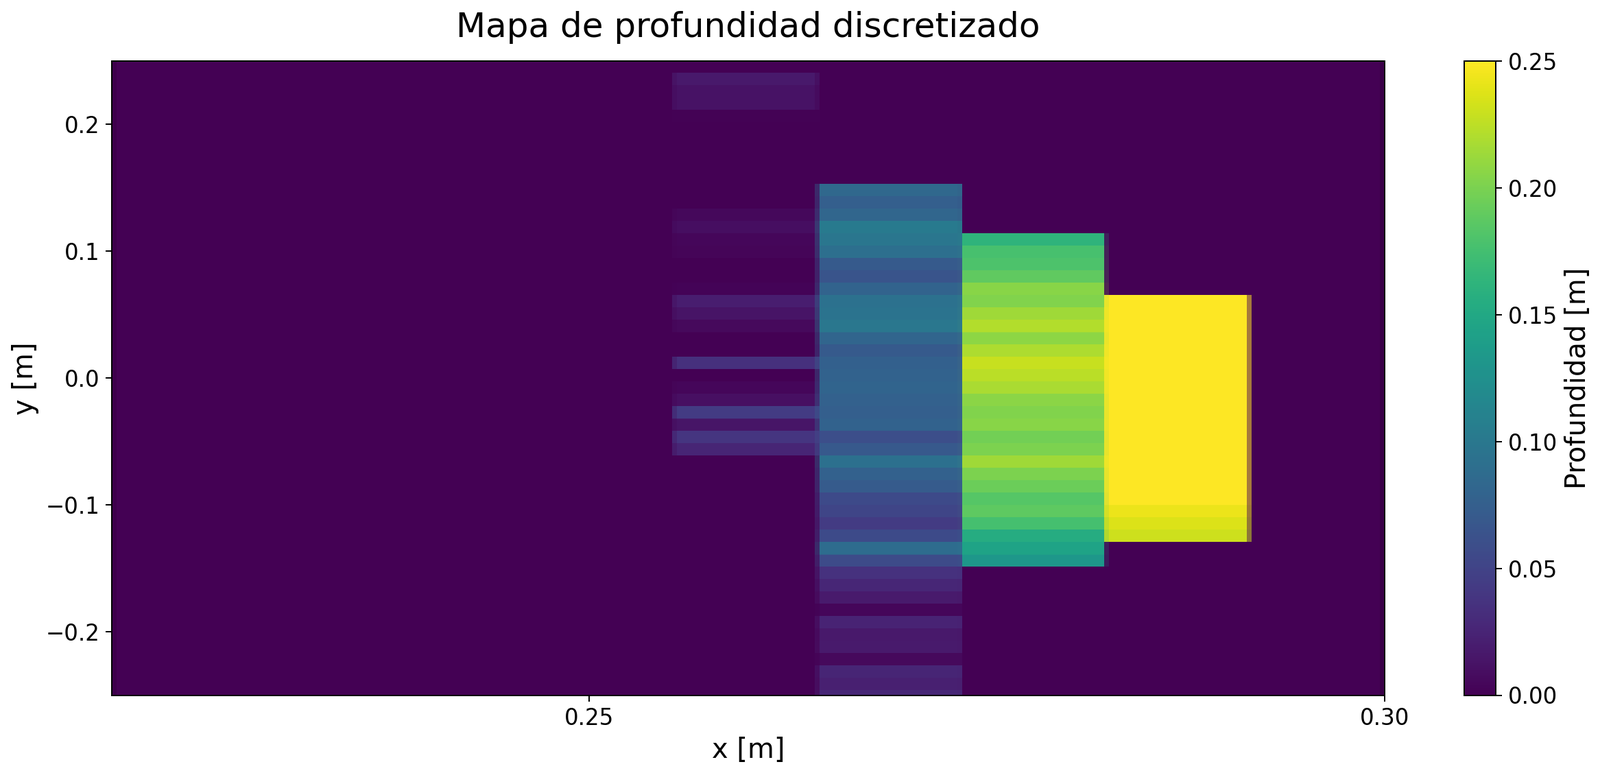
\includegraphics[width=\linewidth]{img/lidar-depth-map.png}
\captionof{figure}{Mapa de profundidad LiDAR: bache de 1348.73~cm$^3$ en 0.0111~m$^2$.}
\end{minipage}

\vfill
\rolebox{Integración de \textbf{hardware electrónico}, arquitectura embebida y \textbf{comunicación entre módulos} (UART, WSS/JSON),
integración de sensores y actuadores, y la \textbf{interfaz web de monitoreo}. Co-autor del manuscrito (ESP32 publicado en GitHub: 8 módulos de firmware, protocolos y hardware documentados).}
\newpage

% =====================================================================
%  PROYECTO 2 — CUBESAT
% =====================================================================
\projecthead{02}{CubeSat 1U — Monitoreo ambiental y telemetría LoRa}
  {Equipo \emph{Arquitectos Galácticos} \;|\; 1.ª Competencia Nacional de Pequeños Satélites 2024 (INRAS-PUCP, VRI-PUCP, CONIDA)}

\metricstrip{17}{equipos finalistas}{100 m}{caída libre desde dron}{6 sensores}{I\textsuperscript{2}C + UART, 21 variables}{2 PCB}{diseñadas en EasyEDA}

\begin{minipage}[t]{0.545\linewidth}
\vspace{0pt}
\sect{Descripción}
Satélite 1U lanzado desde un dron a 100~m y liberado en caída libre. Un \textbf{ESP32} adquiere temperatura, presión, humedad,
aceleración, giro, campo magnético, tensión/corriente y posición GPS; los empaqueta en \textbf{JSON} y los transmite por
\textbf{LoRa (SX1278, 433~MHz)} a una estación terrena con interfaz gráfica en tiempo real. Al descender, el sistema
\textbf{libera el paracaídas} mediante dos servos SG90.

\sect{Detalles técnicos}
\textbf{Altitud relativa} desde el BME280 (fórmula barométrica internacional, referenciada al suelo de arranque $h_0$):
\begin{equation}
  h = \frac{1-\left(P/1013.25\right)^{1/5.2559}}{2.25577\times10^{-5}} - h_0 \quad[\mathrm{m}],\; P\text{ en hPa}
\end{equation}
\textbf{Lógica de despliegue con histéresis} (evita disparos por ruido): el sistema se \emph{arma} al superar $85$~m y
\emph{despliega} (servos a $90^\circ$) cuando, ya armado, desciende por debajo de $80$~m:
\begin{align}
  \text{armado}&\leftarrow \text{armado}\lor(h>85)\\
  \text{despliegue}&=\text{armado}\land(h<80)
\end{align}
\textbf{Paquetización LoRa}: el JSON se fragmenta en $N=\lceil L/50\rceil$ paquetes de hasta 50 caracteres con 50~ms entre
paquetes; el receptor reensambla y extrae cada variable con \texttt{sscanf}.

\renewcommand{\arraystretch}{1.12}\footnotesize
\begin{tabularx}{\linewidth}{@{}>{\bfseries}lXl@{}}
\toprule
Módulo & Función & Bus\\\midrule
ESP32 DevKit V1  & MCU dual-core 240~MHz, 520~KB SRAM        & ---\\
BME280           & Presión, temperatura, humedad ($-40$..$85\,^\circ$C) & I\textsuperscript{2}C\\
MPU6050          & Acel. $\pm16$~g + giroscopio, ADC 16 bits   & I\textsuperscript{2}C\\
QMC5883L         & Magnetómetro 3 ejes ($\pm8$~G), calibrado   & I\textsuperscript{2}C\\
INA219           & Corriente/tensión (resol. 0.8~mA / 4~mV)    & I\textsuperscript{2}C\\
NEO-6M           & GPS, 50 canales, $-161$~dBm                 & UART\\
SX1278 (Ra-02)   & LoRa $+20$~dBm, hasta $-148$~dBm            & SPI\\\bottomrule
\end{tabularx}

\sect{Calibración y pruebas}
\small
\textbf{Magnetómetro}: corrección de \emph{offset} y escala por eje, $m_c=s\odot(m-b)$, con
$b=(-276,\,269,\,-348)$ y $s=(1.08,\,1.11,\,0.86)$; el acimut se obtiene de $m_c$.
\begin{itemize}
  \item Pausa de 500~ms entre ciclos de adquisición y transmisión, con reintentos de inicialización de cada sensor.
  \item Prueba de telemetría con antenas helicoidales y pruebas térmicas en el INRAS, visualizadas en tiempo real en la GUI de estación terrena.
\end{itemize}
\end{minipage}\hfill
\begin{minipage}[t]{0.435\linewidth}
\vspace{0pt}
\centering
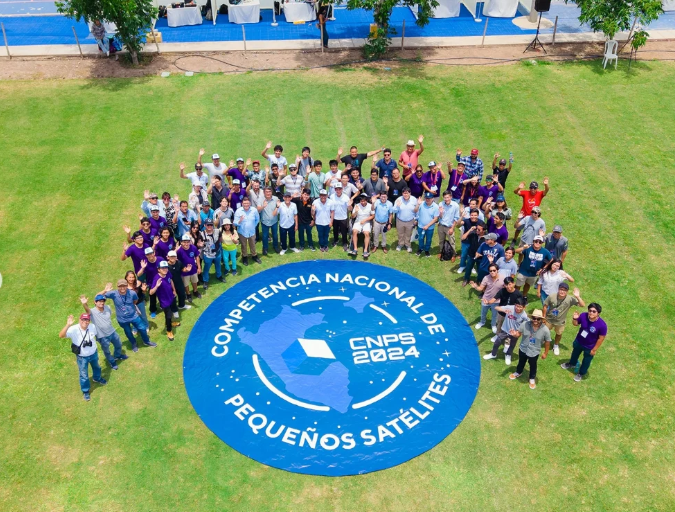
\includegraphics[width=\linewidth]{img/cs_GWN2etC.png}
\captionof{figure}{Fase final de la competencia (CNPS 2024).}
\vspace{3pt}
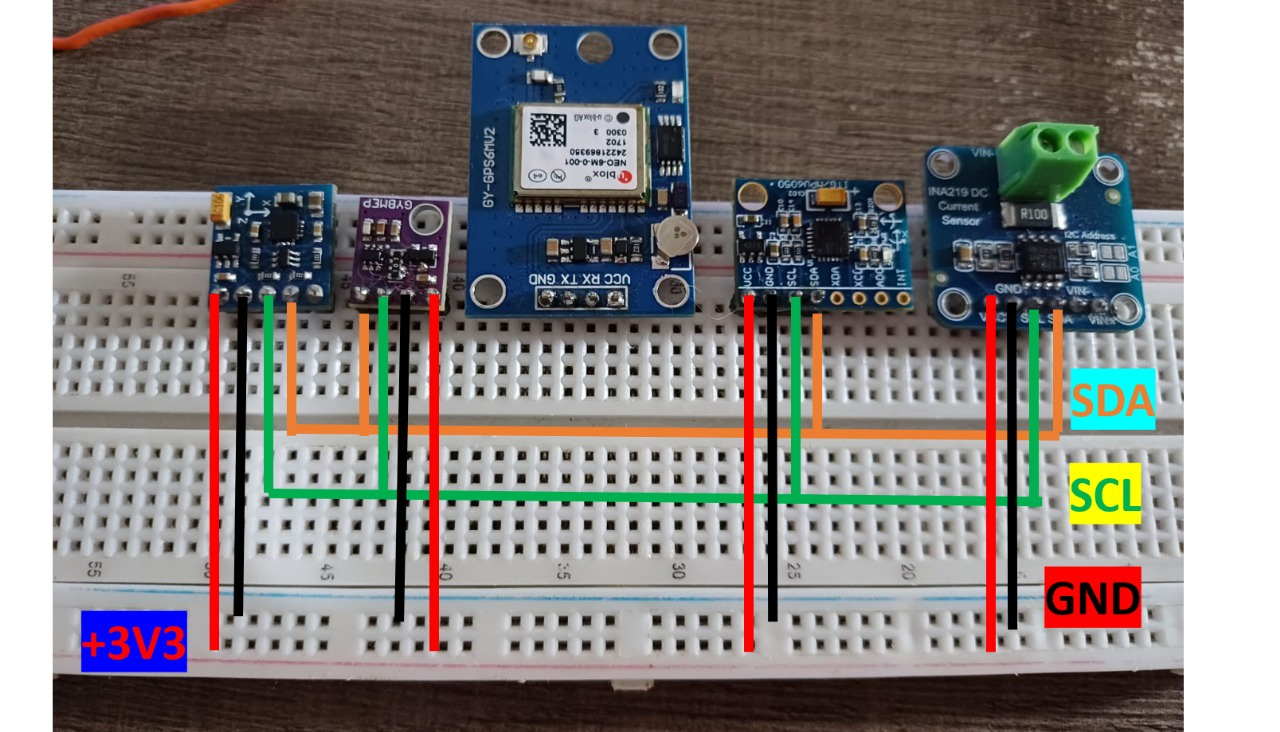
\includegraphics[width=\linewidth]{img/cs_Cmlhuhz.jpeg}
\captionof{figure}{Validación en protoboard: bus I\textsuperscript{2}C común (SDA/SCL/3V3/GND) y GPS.}
\vspace{3pt}
\begin{minipage}[t]{0.485\linewidth}\centering
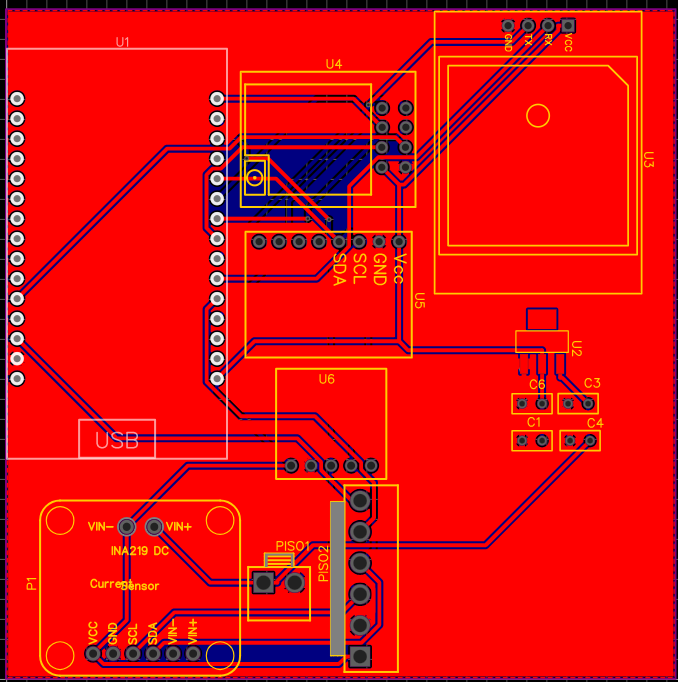
\includegraphics[width=\linewidth]{img/cs_Q54q2ht.png}
\captionof{figure}{PCB piso 2: ESP32, GPS, LoRa, IMU.}
\end{minipage}\hfill
\begin{minipage}[t]{0.485\linewidth}\centering
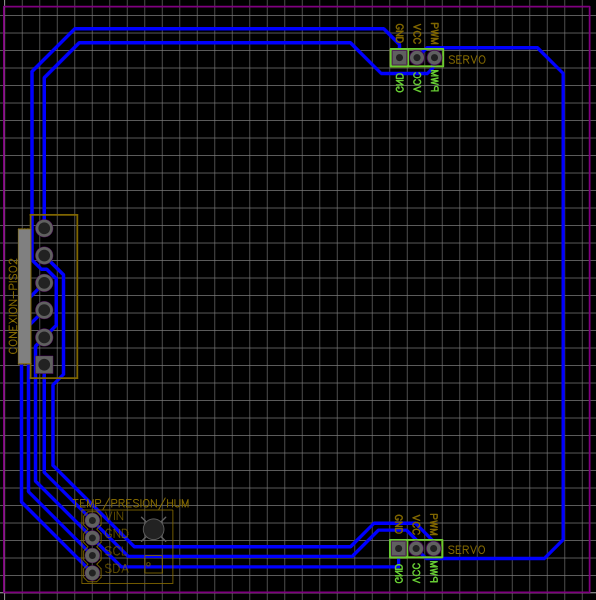
\includegraphics[width=\linewidth]{img/cs_EGLJfHs.png}
\captionof{figure}{PCB piso 3: BME280 y servos.}
\end{minipage}
\end{minipage}

\vfill
\rolebox{\textbf{Selección de componentes} (matriz morfológica, diagrama de flujo, criterios de precio/disponibilidad/viabilidad),
\textbf{firmware en C++ para ESP32} (adquisición de todos los sensores y transmisión LoRa), \textbf{esquemáticos y PCB} en EasyEDA
respetando las dimensiones del CubeSat. \emph{Lección aprendida}: para una siguiente iteración, baterías Li-Ion de 3.7~V en lugar de pilas alcalinas y un mecanismo de despliegue más robusto.}
\newpage

% =====================================================================
%  PROYECTO 3 — ARPEGGIATOR
% =====================================================================
\projecthead{03}{ESP32-S3 Arpeggiator — Instrumento musical digital autónomo}
  {Síntesis digital $\cdot$ audio I\textsuperscript{2}S $\cdot$ PCB y gabinete propios \;|\; Diseño Electrónico 2 (1IEE17, 2024-2), PUCP \;|\; Asesor: H.~Pratt}

\metricstrip{13}{notas (C4--C5), 3 ondas, 3 modos}{16 bit}{I\textsuperscript{2}S a 44.1~kHz}{+15}{iteraciones de firmware y hardware}{13 LED}{WS2812B de realimentación}

\begin{minipage}[t]{0.545\linewidth}
\vspace{0pt}
\sect{Descripción}
Instrumento independiente basado en un \textbf{ESP32-S3}: el usuario selecciona cualquier combinación de notas en un teclado de una
octava y el equipo las reproduce como arpegio \emph{ascendente, descendente o aleatorio}, con onda senoidal, cuadrada o triangular,
velocidad y tono ajustables por potenciómetro. El audio sale por \textbf{I\textsuperscript{2}S} hacia un DAC PCM5102 y un amplificador clase D TPA3116D2.

\sect{Detalles técnicos}
\textbf{Cadena de señal:}
\vspace{2pt}

\centering
\begin{tikzpicture}[x=1cm,y=1cm,
  blk/.style={draw=accent,fill=soft,rounded corners=1.5pt,minimum height=0.62cm,inner sep=2.5pt,font=\fontsize{6.5}{7}\selectfont,align=center},
  arr/.style={-{Stealth[length=3pt]},draw=accent2,thick}]
  \node[blk] (a) {Teclado\\13 notas};
  \node[blk,right=0.28cm of a] (b) {Lista\\ordenada};
  \node[blk,right=0.28cm of b] (c) {LUT 256\\+ tono};
  \node[blk,right=0.28cm of c] (d) {Filtro\\IIR};
  \node[blk,right=0.28cm of d] (e) {I\textsuperscript{2}S\\DAC};
  \node[blk,right=0.28cm of e] (f) {Amp.\\+ altavoz};
  \foreach \s/\t in {a/b,b/c,c/d,d/e,e/f}{\draw[arr] (\s) -- (\t);}
\end{tikzpicture}
\par\vspace{3pt}\raggedright

\textbf{Afinación} con tono continuo $p\in[-0.5,0.5]$ (potenciómetro, ADC de 12 bits), y \textbf{duración} repartida entre las notas activas:
\begin{equation}
  f_\mathrm{aj}=f_0\cdot2^{\,p},\qquad
  T_\mathrm{nota}=\frac{T_\mathrm{ciclo}}{N_\mathrm{activas}}
\end{equation}
\textbf{Oscilador por tabla (LUT)}: 256 muestras por forma de onda ($x[m]=32767\sin(2\pi m/256)$ para la senoidal), con $f_s=44.1$~kHz y bloques de 64 muestras:
\begin{equation}
  N_p=\left\lfloor \frac{f_s}{f_\mathrm{aj}}\right\rfloor,\qquad
  i[n]=\left\lfloor\frac{(n \bmod N_p)\cdot 256}{N_p}\right\rfloor
\end{equation}
\textbf{Filtro de suavizado} de primer orden (estado persistente entre bloques y notas), con coeficiente $a\in[0,1]$:
\begin{equation}
  y[n]=y[n-1]+a\,\big(x[n]-y[n-1]\big)
\end{equation}

\renewcommand{\arraystretch}{1.12}\footnotesize
\begin{tabularx}{\linewidth}{@{}>{\bfseries}lXl@{}}
\toprule
Subsistema & Implementación & GPIO\\\midrule
Audio I\textsuperscript{2}S & BCLK / LRCLK / DATA $\to$ PCM5102 & 4 / 5 / 18\\
Notas (C4--C5) & 13 pulsadores con \emph{toggle} y LED por nota & 8, 12--17, 19--21, 35--37\\
Controles & Velocidad y tono (ADC), modo y onda (botones) & 3, 10, 40, 39\\
LEDs & Cadena de 13 WS2812B (un hilo) & 38\\\bottomrule
\end{tabularx}

\sect{Lecciones y mejoras previstas}
\small
\begin{itemize}
  \item \textbf{Hardware}: la huella del ESP32-S3 en la PCB no encajó como se esperaba y el gabinete resultó más alto de lo necesario; una 2.\textsuperscript{a} revisión corrige huellas, orificios de montaje y cableado de pulsadores.
  \item \textbf{Firmware}: reproducción bloqueante y \texttt{delay()} como antirrebote $\to$ máquina de estados con \texttt{millis()}, audio por DMA/tarea FreeRTOS, DDS con acumulador de fase y envolvente ADSR.
\end{itemize}
\end{minipage}\hfill
\begin{minipage}[t]{0.435\linewidth}
\vspace{0pt}
\centering
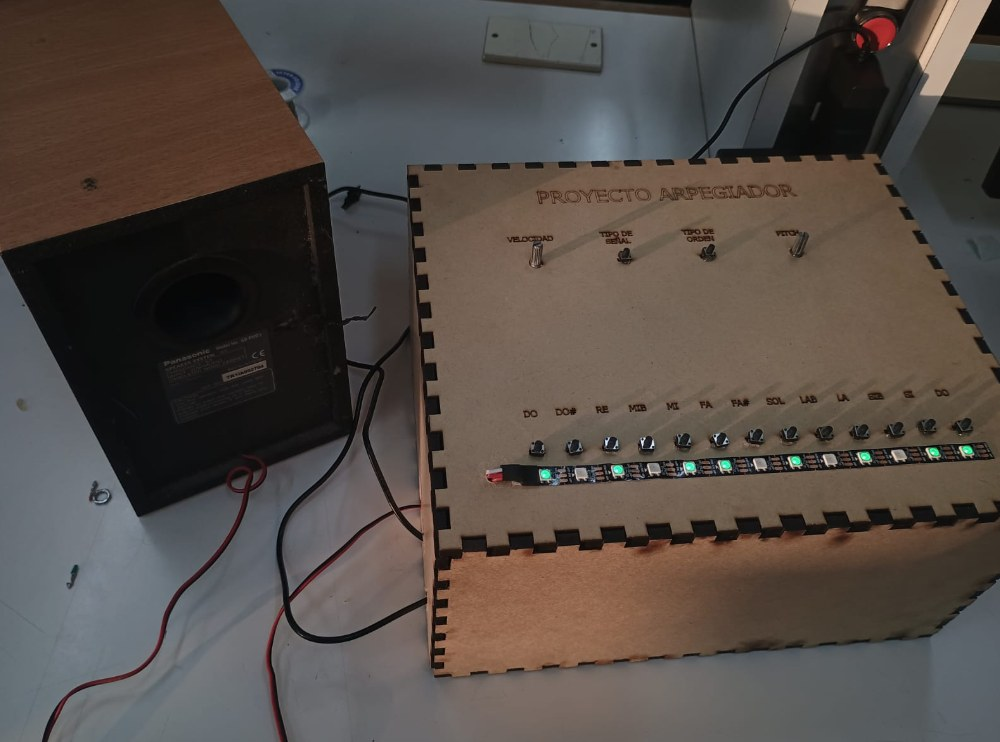
\includegraphics[width=\linewidth]{img/arp_final-prototype.jpg}
\captionof{figure}{Prototipo final: gabinete MDF de 5.5~mm ($\approx$25$\times$30$\times$15~cm), LEDs de nota y altavoz.}
\vspace{3pt}
\begin{minipage}[t]{0.485\linewidth}\centering
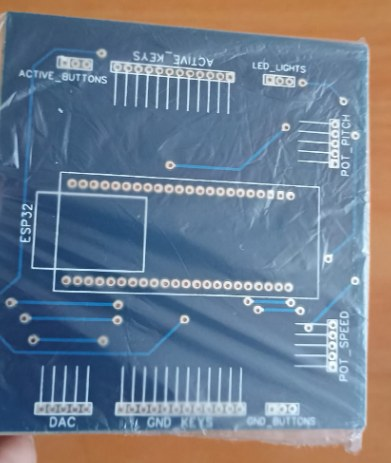
\includegraphics[width=\linewidth,height=3.9cm,keepaspectratio]{img/arp_fabricated-pcb.jpg}
\captionof{figure}{PCB doble capa fabricada.}
\end{minipage}\hfill
\begin{minipage}[t]{0.485\linewidth}\centering
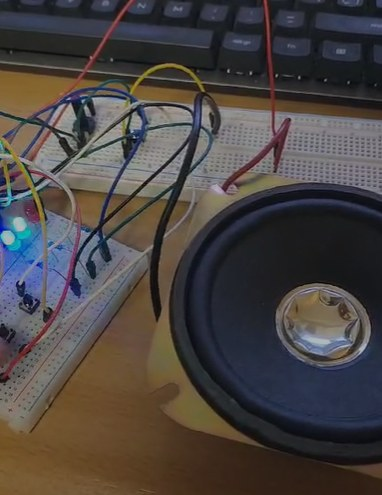
\includegraphics[width=\linewidth,height=3.9cm,keepaspectratio]{img/arp_dac-audio-test.jpg}
\captionof{figure}{Prueba DAC + amplificador.}
\end{minipage}
\vspace{3pt}
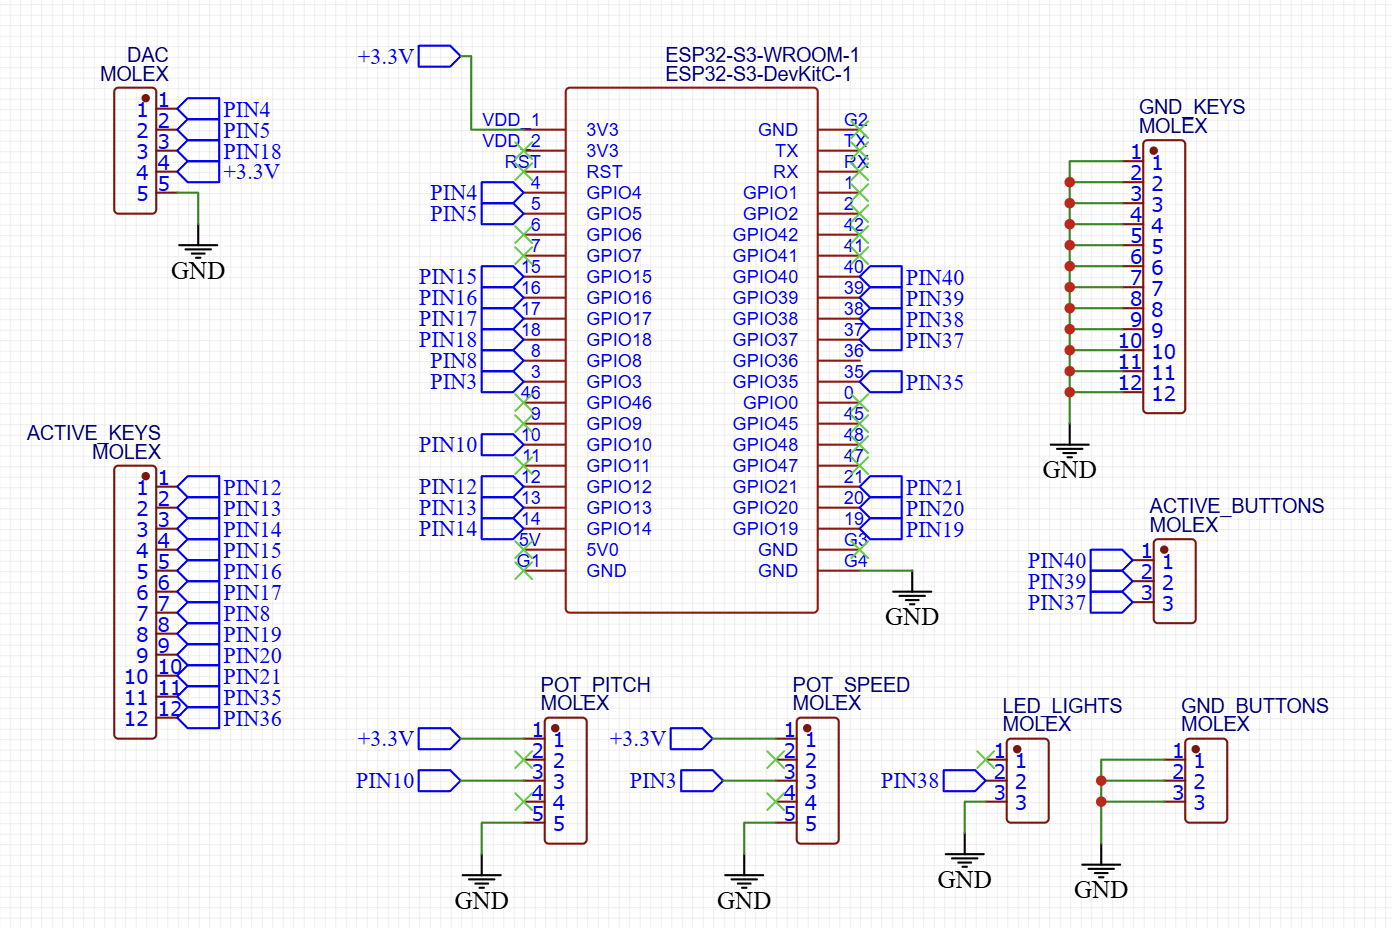
\includegraphics[width=\linewidth]{img/arp_hardware-schematic.png}
\captionof{figure}{Esquemático: ESP32-S3 y conectores Molex.}
\end{minipage}

\vfill
\rolebox{Integrante del equipo de 4 estudiantes (M.~Bruschi, R.~Yupanqui, E.~Torres, J.~López). Flujo completo \textbf{idea $\to$ prototipo $\to$ producto}:
prueba de DAC con senoidal de 400~Hz, prototipo PWM, migración a I\textsuperscript{2}S, \textbf{diagnóstico y eliminación del ruido intermitente
(\emph{popcorn})} reescribiendo la generación de muestras, PCB propia y gabinete cortado en láser.
Repositorio con \textbf{revisión de código} documentada: límites conocidos (reproducción bloqueante, \texttt{delay()} como antirrebote) y plan de mejora
(acumulador de fase/DDS, sincronización con \texttt{millis()}, envolvente ADSR, MIDI).}
\end{document}
